Figure \ref{fig:disjoint} shows a typical program fragment that
highlights some aspects of program execution that our microarchitecture
can address.
Mainline path execution (the most predicted path) is shown with the
solid bold control flow edges.  Opportunities for the spawning of alternative
speculative paths (disjoint paths) are shown with the lighter dashed
control flow edges.  In this example, two simple, single-sided hammock 
branches are shown in the body of the loop.  One is predicted as
being taken.  The other is predicted to fall through.  Our microarchitecture
will try to exploit both types of conditional branches by capturing
and speculatively executing
all of the instructions in the body of this loop (given this particular
case).  This is possible due to the ability of the microarchitecture to
both execute large numbers of instructions speculatively but also
because our microarchitecture is specially suited towards handling
issues related to multipath execution.
%
\begin{figure}
\centering
\epsfig{file=disjoint.eps,width=4.5in}
\caption{{\em Example Program Showing Predicted and Disjoint
Paths.} 
This example shows both the predicted path through the program 
(in bold) as
well as where alternative speculative disjoint paths may be
spawned (dashed).}
\label{fig:disjoint}
\end{figure}

